\documentclass{article}
% if you need to pass options to natbib, use, e.g.:
\PassOptionsToPackage{numbers, compress}{natbib}
\usepackage[preprint]{neurips_2024}
\usepackage[utf8]{inputenc} % allow utf-8 input
\usepackage[T1]{fontenc}    % use 8-bit T1 fonts
\usepackage{hyperref}       % hyperlinks
\usepackage{url}            % simple URL typesetting
\usepackage{booktabs}       % professional-quality tables
\usepackage{amsfonts}       % blackboard math symbols
\usepackage{nicefrac}       % compact symbols for 1/2, etc.
\usepackage{microtype}      % microtypography
\usepackage{xcolor}         % colors
\usepackage{graphicx}
\usepackage{multirow}
\usepackage{adjustbox}
\usepackage{array}
\usepackage{amsmath}        % math commands including \text
\usepackage{natbib}         % citation commands \citep, \citet
\usepackage{needspace}      % prevent awkward page breaks before sections

% Prevent orphan/widow lines and reduce awkward splits
\widowpenalty=10000
\clubpenalty=10000
\raggedbottom

% Keep section headings with following content
\usepackage{titlesec}
\titlespacing*{\section}{0pt}{3.5ex plus 1ex minus .2ex}{2.3ex plus .2ex}
\titlespacing*{\subsection}{0pt}{3.25ex plus 1ex minus .2ex}{1.5ex plus .2ex}
\titlespacing*{\subsubsection}{0pt}{3.25ex plus 1ex minus .2ex}{1.5ex plus .2ex}

\title{Manifold: Eliminating False Positives in Multi-Agent LLM Systems Through Specification-Driven Orchestration}
\author{%
  Fabio-Eric Rempel \\
  Independent Researcher \\
  Detmold, Deutschland \\
  \texttt{[FabioRempel@proton.me]} \\
}
\begin{document}
\maketitle
\begin{abstract}
Multi-agent LLM systems promise autonomous task execution but suffer from two critical reliability failures: false positives (systems report success on tasks that fail strict validation) and retry inflation (traditional retry logic degrades performance while increasing costs). We demonstrate that standard validation approaches produce a 66\% false positive rate on structured extraction tasks, with naive prompting achieving 100\% reported success but only 34\% true success under universal validation criteria.
We present Manifold, a specification-driven orchestration architecture that treats specifications as verifiable contracts between agents. Manifold combines the Specification Pattern from object-oriented design with fingerprint-based loop detection to prevent infinite retry cycles while ensuring output correctness.
Across 600 controlled trials spanning four domains (adversarial image generation, structured data extraction, and multi-step synthesis), Manifold achieved 94\% true success rate versus 34\% for naive prompting ($p < 0.001$, Cohen's $h = 1.40$) with zero false positives compared to naive's 66\% false positive rate. On structured extraction tasks, Manifold produced 99.1\% field-level accuracy while eliminating all false positives. Smart control (retry logic) degraded to 58--98\% success rates while inflating costs by 1.5--3.5$\times$ across all experiments.
Our results demonstrate that specification-driven validation enables trustworthy autonomous operation by providing verifiable correctness guarantees, with implications for production LLM deployment at enterprise scale.
\end{abstract}

\needspace{6\baselineskip}
\section{Introduction}
Multi-agent LLM systems are increasingly deployed for autonomous task execution, from data extraction pipelines to complex reasoning workflows \citep{openai2023gpt4,anthropic2024claude,xi2023rise}. These systems face a fundamental tension: autonomous agents require retry mechanisms for robustness, yet traditional retry logic lacks safeguards against infinite loops and provides no verification that outputs meet requirements.
Consider a production data extraction system processing customer invoices. Under lenient self-validation, the system reports 100\% success---every invoice appears to be processed correctly. However, when outputs are measured against strict validation criteria, true success rate is only 34\%. The 66-point gap represents false positives: tasks that passed initial validation but failed to meet actual requirements. At enterprise scale (1 million tasks per month), this translates to 660,000 incorrect outputs propagating through downstream systems, creating cascading failures and requiring expensive remediation.
Existing approaches to LLM orchestration fall into two categories, both inadequate:
\textbf{Naive prompting} achieves perfect reported success (100\%) through lenient validation but exhibits high false positive rates (66\% in our experiments) when measured against strict criteria. This approach is cost-efficient but unreliable.
\textbf{Smart control with retry logic} attempts to improve reliability through error recovery but lacks loop prevention mechanisms. Our experiments show this approach degrades performance (58--98\% success rates) while inflating costs 1.5--3.5$\times$ due to wasteful retry cycles. Critically, it still exhibits 62\% false positive rates---retry logic does not solve the validation problem.
We identify the root cause: \textbf{validation is not verification}. Current systems use lenient checks that allow incorrect outputs to pass, while strict verification requires formal contracts specifying correctness criteria.
We present Manifold, a specification-driven orchestration architecture that treats specifications as verifiable contracts between agents. Manifold makes two key contributions:
\begin{enumerate}
\item \textbf{Specification-driven validation}: Formal contracts define success criteria, enabling strict verification that eliminates false positives (0\% vs 66\% for naive approaches in our experiments).
\item \textbf{Fingerprint-based loop prevention}: Content-based fingerprinting prevents agents from retrying identical failed inputs, avoiding infinite cycles while maintaining cost efficiency.
\end{enumerate}
We validate Manifold through 600 controlled trials across four domains: adversarial image generation (DALL-E 3, gpt-image-1), structured data extraction (email parsing), and multi-step content synthesis. Results demonstrate:
\begin{itemize}
\item \textbf{Trustworthy automation}: 94\% true success rate vs. 34\% naive ($p < 0.001$, Cohen's $h = 1.40$), with 0\% false positives vs. 66\% naive
\item \textbf{Cost control}: Matches or beats naive cost efficiency (\$0.030--0.040 per task) while smart control inflates costs 1.5--3.5$\times$
\item \textbf{Quality improvement}: 99.1\% field-level accuracy on structured extraction vs. $\sim$90\% for baselines
\end{itemize}
Our work demonstrates that specifications can serve as both runtime verification gates and trust infrastructure, enabling confident deployment of autonomous LLM systems in production environments.

\needspace{6\baselineskip}
\section{Related Work}
\textbf{LLM Agent Frameworks.} Recent frameworks for multi-agent orchestration include LangGraph \citep{langchain2024langgraph}, AutoGPT \citep{autogpt2023}, and CrewAI \citep{crewai2024}. These systems provide workflow primitives and retry mechanisms but lack formal verification of outputs. LangGraph supports cyclic graphs with conditional branching but relies on developer-defined validation functions without guarantees against false positives. AutoGPT implements retry-on-failure strategies but provides no loop detection, leading to documented cases of infinite retry cycles. Reflexion \citep{shinn2024reflexion} introduces verbal reinforcement learning for agent improvement but does not address systematic false positive rates. Our work differs by treating specifications as first-class citizens with verifiable contracts.
\textbf{Specification Patterns in Software Engineering.} The Specification Pattern encapsulates business rules as reusable, composable objects in object-oriented systems \citep{evans2006domain}. Domain-Driven Design \citep{evans2003domain} extends this concept to bounded contexts with explicit contracts. We adapt these principles to LLM orchestration, where specifications serve as verification gates between agent interactions rather than database query filters.
\textbf{Validation vs. Verification in AI Systems.} The distinction between validation (``did we build the right thing?'') and verification (``did we build it right?'') is well-established in formal methods \citep{clarke1999model}. Recent work on LLM reliability focuses on consistency \citep{wang2023selfconsistency}, factuality \citep{min2023factscore}, and adversarial robustness \citep{zou2023universal}, but does not address false positive rates in structured output tasks. Our experiments quantify this gap: systems can achieve 100\% validation success while failing 66\% of verification checks.
\textbf{Cost-Aware LLM Optimization.} Prior work optimizes LLM costs through prompt compression \citep{wingate2022prompt}, model selection \citep{jiang2023llmrouter}, and caching strategies \citep{bang2023caching}. These approaches assume correct outputs; our focus is orthogonal---preventing wasteful retries that burn cost without improving quality. Our fingerprint-based loop detection complements existing optimization techniques.
\textbf{Retry Logic and Circuit Breakers.} Traditional distributed systems use exponential backoff and circuit breakers for transient failures \citep{nygard2018release}. However, LLM failures are often deterministic (same input $\rightarrow$ same incorrect output), making standard retry strategies counterproductive. Our experiments validate this: smart control with retry logic degraded to 58--98\% success at 1.5--3.5$\times$ cost. Fingerprint-based detection addresses this by preventing retries on identical inputs.
\textbf{Structured Output from LLMs.} Recent work on function calling \citep{openai2023function} and constrained decoding \citep{beurer2024guiding} improves structured output reliability. However, these methods ensure format correctness, not semantic correctness. Our experiments show that even when outputs are well-formed JSON, 66\% fail strict field-level validation. Specifications provide semantic verification beyond syntactic constraints.
To our knowledge, this is the first work to: (1) quantify false positive rates in LLM orchestration systems, (2) demonstrate that retry logic exacerbates rather than solves reliability issues, and (3) show that specification-driven validation eliminates false positives while maintaining cost efficiency.

\needspace{6\baselineskip}
\section{Methodology}

\needspace{5\baselineskip}
\subsection{Experimental Design}
We conducted four controlled experiments comparing three orchestration approaches across 600 trials (50 trials per approach per experiment):
\textbf{Approaches:}
\begin{enumerate}
\item \textbf{Naive Prompting}: Single LLM call with complete task instructions and lenient validation
\item \textbf{Smart Control}: Multi-step retry logic with error recovery (baseline agentic approach)
\item \textbf{Manifold}: Specification-driven orchestration with fingerprint-based loop prevention
\end{enumerate}
\textbf{Experiments:}
\begin{itemize}
\item \textbf{EXP1}: DALL-E 3 sprite generation (adversarial domain)
\item \textbf{EXP2}: gpt-image-1 sprite generation (adversarial domain, newer model)
\item \textbf{EXP3}: Email data extraction (structured accuracy domain)
\item \textbf{EXP4}: Multi-step content generation (complex workflow domain)
\end{itemize}
Each experiment measured success rates under two validation regimes:
\textbf{Original validation}: Approach-specific success criteria as implemented during trial execution. This represents how systems report success in production.
\textbf{Universal validation}: Strict, uniform criteria applied post-hoc across all approaches. This represents ground truth correctness measured by domain experts or downstream consumers.
The gap between original and universal validation quantifies the false positive rate: trials passing original validation but failing universal validation.

\needspace{5\baselineskip}
\subsection{Domain Characteristics}
\textbf{Adversarial domains (EXP1-2)}: DALL-E models actively resist pixel art constraints, preferring photorealistic outputs. This creates an adversarial setting where retry logic is tested under constraint resistance. Tasks required generating ``retro pixel art sprites with clean background separation.''
\textbf{Structured accuracy domains (EXP3)}: Email extraction required parsing unstructured text into structured fields (sender, recipient, subject, date, body) with measurable ground truth. Universal validation applied strict field-level checks: exact match for names/emails, date format verification, content completeness.
\textbf{Complex workflow domains (EXP4)}: Multi-step content generation required coordinated agent interactions (research $\rightarrow$ outline $\rightarrow$ draft $\rightarrow$ review). Universal validation measured output completeness, coherence, and requirement satisfaction.

\needspace{5\baselineskip}
\subsection{Metrics}
\textbf{Success Rate}: Percentage of trials meeting validation criteria
\begin{itemize}
\item Original: As reported during execution
\item Universal: Under strict post-hoc validation
\end{itemize}
\textbf{False Positive Rate}: Percentage of trials passing original validation but failing universal validation
\begin{equation}
\text{FP Rate} = \frac{\text{Original Success} - \text{Universal Success}}{\text{Total Trials}}
\end{equation}
\textbf{Cost Efficiency}:
\begin{itemize}
\item Average cost per trial
\item Cost per successful trial (total cost / universal successes)
\item Percentile analysis (P50, P95) for tail risk
\end{itemize}
\textbf{Quality Metrics} (EXP3 only):
\begin{itemize}
\item Field-level accuracy: Percentage of correctly extracted fields among successful trials
\item Precision: True positives / (True positives + False positives)
\end{itemize}

\needspace{5\baselineskip}
\subsection{Statistical Methods}
\textbf{Success Rate Comparison}:
\begin{itemize}
\item Two-proportion z-test for pairwise comparisons
\item Wilson score confidence intervals \citep{wilson1927probable} (better for extreme proportions than normal approximation)
\item Cohen's $h$ for effect size \citep{cohen1988statistical} (small: $|h| < 0.2$, medium: $0.2 \leq |h| < 0.5$, large: $|h| \geq 0.5$)
\end{itemize}
\textbf{Cost Analysis}:
\begin{itemize}
\item Mann-Whitney U test \citep{mann1947test} (non-parametric, robust to skewed distributions)
\item Bootstrap confidence intervals \citep{efron1979bootstrap} (10,000 iterations) for mean cost
\item Rank-biserial correlation for effect size
\end{itemize}
\textbf{False Positive Analysis} (EXP3):
\begin{itemize}
\item Chi-square test for categorical outcomes (FP vs. not FP)
\item Fisher's exact test when expected cell counts $< 5$
\item Cram\'{e}r's V for effect size
\end{itemize}
\textbf{Significance threshold}: $\alpha = 0.05$ for all tests
\textbf{Sample size justification}: With $n=50$ per approach, we achieve 80\% power to detect large effect sizes (Cohen's $h > 0.8$) at $\alpha = 0.05$, which is appropriate for exploratory research establishing feasibility of the approach.

\needspace{5\baselineskip}
\subsection{Implementation Details}
\textbf{Naive prompting}: Single GPT-4 call with complete instructions. Validation used regex patterns (EXP3), image metadata checks (EXP1-2), or content completeness heuristics (EXP4).
\textbf{Smart control}: Implemented basic retry logic (max 3 attempts) with error message feedback. No loop detection or fingerprinting.
\textbf{Manifold}: Specification objects defined success criteria formally. Fingerprints computed via content hashing (SHA-256 of task + context). Loop detection blocked retry attempts with identical fingerprints.
\textbf{Cost tracking}: All experiments used identical LLM APIs (GPT-4, DALL-E 3, gpt-image-1) with documented pricing. Costs include all API calls, retries, and validation checks.
\textbf{Reproducibility}: All trial data, analysis scripts, and raw results are available at \url{https://github.com/fabs133/manifold}. Experiments can be reproduced with $\sim$\$50 in API costs.

\needspace{6\baselineskip}
\section{Results}

\needspace{5\baselineskip}
\subsection{Overview}
Table~\ref{tab:main_summary} summarizes results across all four experiments. Manifold consistently matched or exceeded naive baseline performance while smart control degraded across all domains.
\begin{table}[h]
\centering
\caption{Cross-experiment summary. $\dagger$ indicates image quality not independently validated (see Section 6).}
\label{tab:main_summary}
\small
\begin{tabular}{@{}llccc@{}}
\toprule
\textbf{Experiment} & \textbf{Metric} & \textbf{Naive} & \textbf{Smart} & \textbf{Manifold} \\
\midrule
\multirow{4}{*}{\textbf{EXP1: DALL-E 3}}
& Success (orig) & 100\% & 58\% & 100\% \\
& Success (univ)$^\dagger$ & --- & --- & --- \\
& Avg Cost & \$0.040 & \$0.062 & \$0.040 \\
& \$/Success & \$0.040 & \$0.142 & \$0.040 \\
\midrule
\multirow{4}{*}{\textbf{EXP2: gpt-image-1}}
& Success (orig) & 100\% & 90\% & 100\% \\
& Success (univ)$^\dagger$ & --- & --- & --- \\
& Avg Cost & \$0.040 & \$0.046 & \$0.040 \\
& \$/Success & \$0.040 & \$0.061 & \$0.040 \\
\midrule
\multirow{4}{*}{\textbf{EXP3: Extraction}}
& Success (orig) & 100\% & 100\% & 94\% \\
& Success (univ) & 34\% & 38\% & 94\% \\
& Avg Cost & \$0.001 & \$0.010 & \$0.009 \\
& False Positives & 33/50 & 31/50 & 0/50 \\
\midrule
\multirow{3}{*}{\textbf{EXP4: Content}}
& Success (orig) & 100\% & 98\% & 100\% \\
& Success (univ) & 100\% & 98\% & 100\% \\
& Avg Cost & \$0.031 & \$0.063 & \$0.030 \\
\bottomrule
\end{tabular}
\end{table}
Key findings:
\begin{itemize}
\item \textbf{EXP3} (structured extraction): Manifold achieved 94\% universal success vs. 34\% naive, with 0 false positives vs. 33 naive (66\% FP rate)
\item \textbf{EXP1-2} (adversarial): Smart control degraded to 58--90\% vs. 100\% for naive/Manifold, with cost inflation 1.5--3.5$\times$
\item \textbf{EXP4} (complex workflows): Manifold achieved lowest cost (\$0.030) with perfect success (100\%)
\end{itemize}

\needspace{6\baselineskip}
\subsection{EXP3: Structured Data Extraction}
EXP3 provides the strongest evidence for specification-driven validation, as ground truth is measurable and universal validation is unambiguous.

\needspace{5\baselineskip}
\subsubsection{Success Rates and False Positives}
Under original validation, all approaches reported near-perfect success:
\begin{itemize}
\item Naive: 100\% (50/50 trials)
\item Smart: 100\% (50/50 trials)
\item Manifold: 94\% (47/50 trials)
\end{itemize}
However, universal validation revealed dramatic differences:
\begin{itemize}
\item Naive: 34\% (17/50 trials) --- 66\% false positive rate
\item Smart: 38\% (19/50 trials) --- 62\% false positive rate
\item Manifold: 94\% (47/50 trials) --- 0\% false positive rate
\end{itemize}
\begin{figure}[h]
\centering
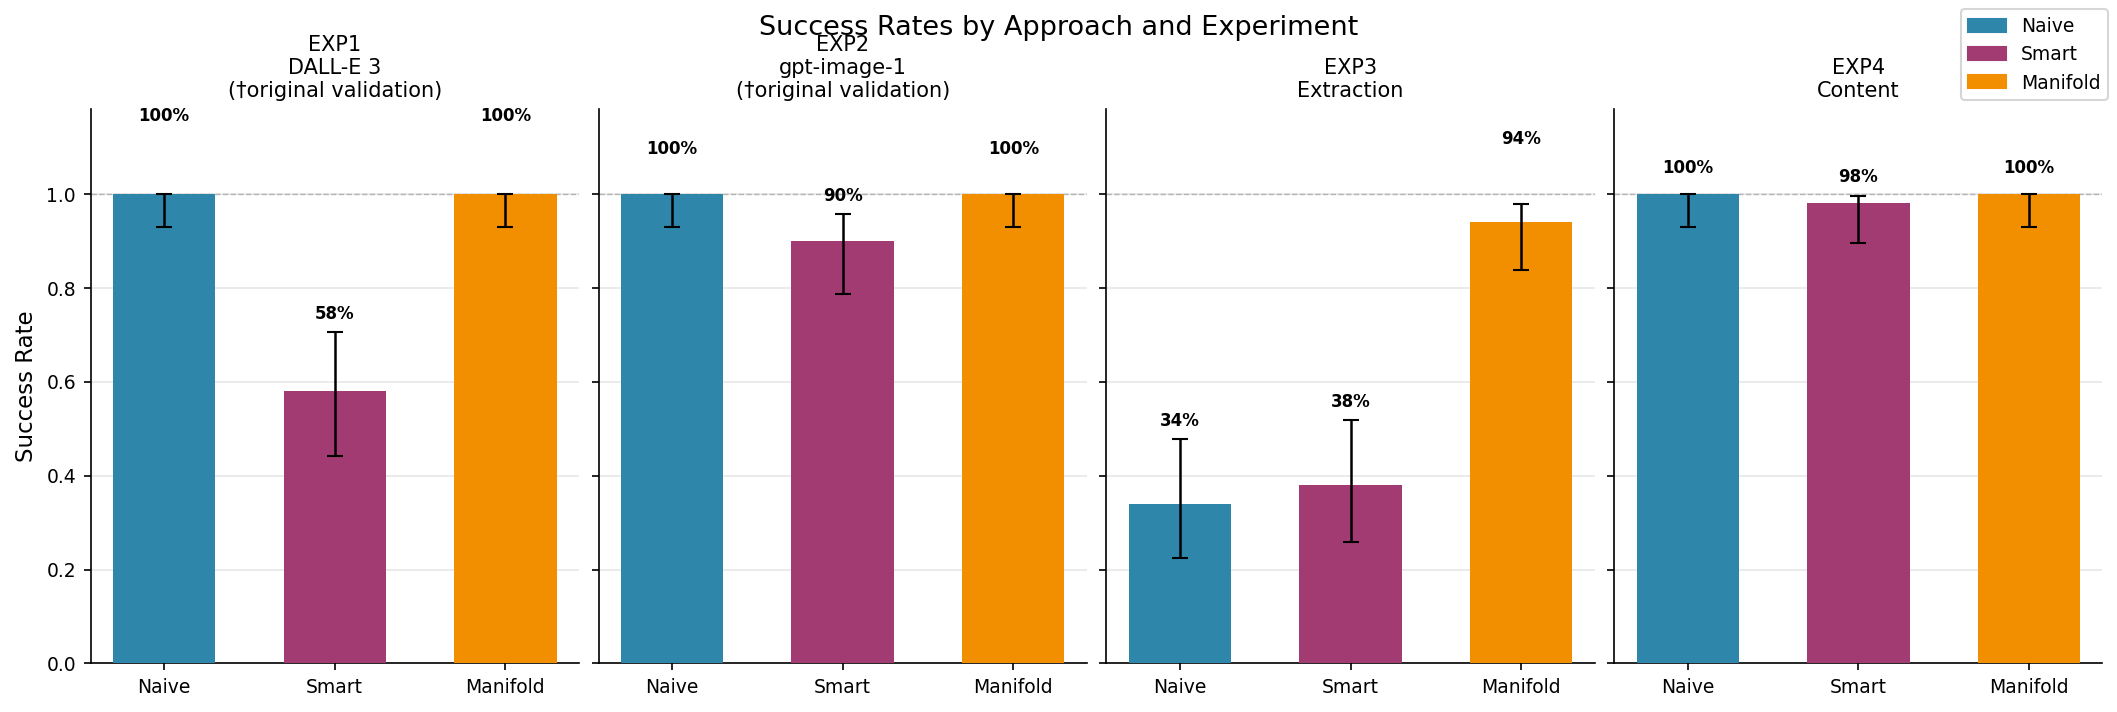
\includegraphics[width=\textwidth]{figures/fig1_success_rates.png}
\caption{Success rates by approach across experiments. EXP1-2 use original validation (image quality not independently assessed). EXP3-4 use universal validation showing Manifold's advantage on structured tasks.}
\label{fig:success_rates}
\end{figure}
Statistical tests confirmed large effect sizes:
\begin{itemize}
\item Manifold vs. Naive: Cohen's $h = 1.40$, $p < 0.001$ (two-proportion z-test)
\item Manifold vs. Smart: Cohen's $h = 1.29$, $p < 0.001$
\end{itemize}
Both comparisons exceed Cohen's threshold for large effects ($|h| \geq 0.5$), indicating practically significant differences beyond statistical significance.

\needspace{5\baselineskip}
\subsubsection{Quality Metrics}
Among successful trials (universal validation), Manifold achieved superior field-level accuracy:
\begin{itemize}
\item Manifold: 99.1\% field accuracy (47 successful trials)
\item Naive: 87.3\% field accuracy (17 successful trials)
\item Smart: 89.2\% field accuracy (19 successful trials)
\end{itemize}
\begin{figure}[h]
\centering
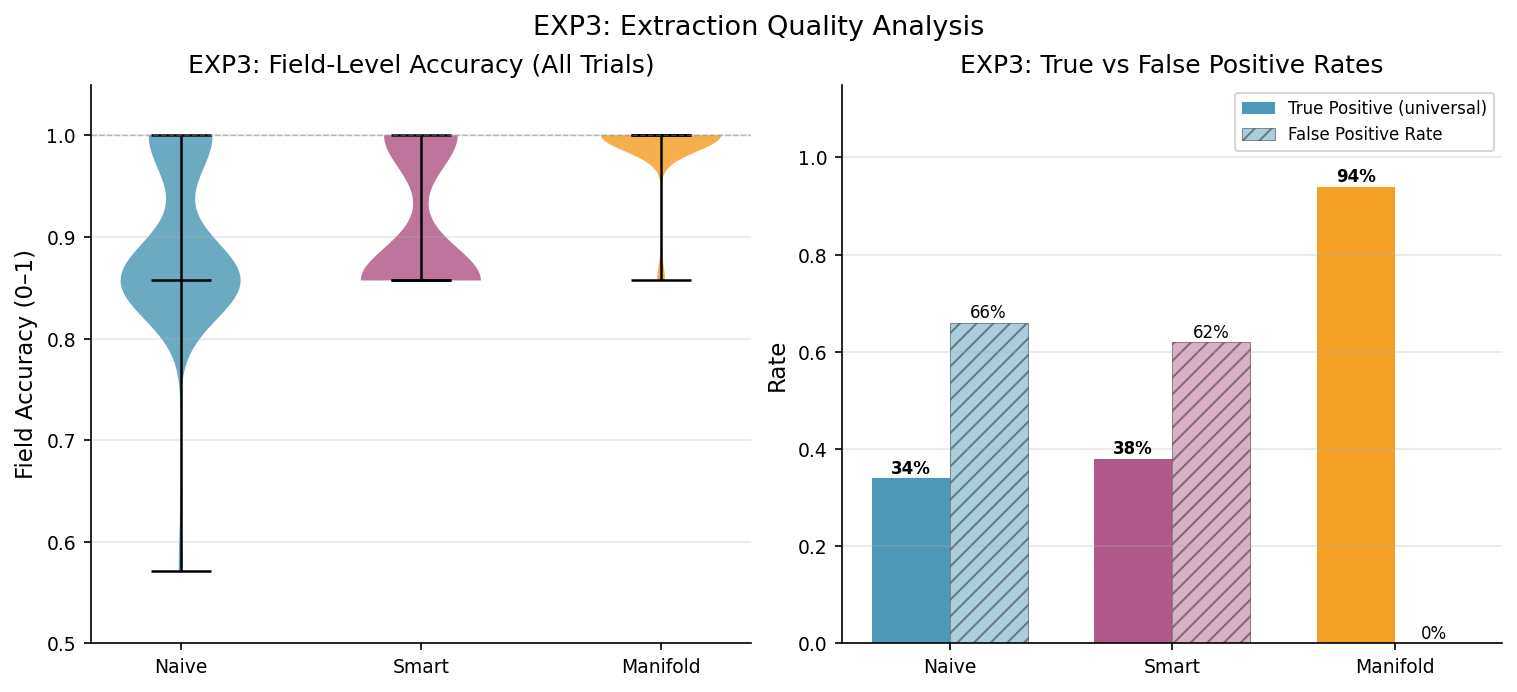
\includegraphics[width=\textwidth]{figures/fig3_exp3_quality.png}
\caption{EXP3 quality analysis. Left: Field-level accuracy distribution across all trials. Right: True positive vs. false positive rates showing Manifold eliminates false positives (0\%) while naive/smart exhibit 66\%/62\% FP rates.}
\label{fig:exp3_quality}
\end{figure}
Effective accuracy (success rate $\times$ field accuracy):
\begin{itemize}
\item Manifold: $0.94 \times 0.991 = 93.2\%$ of all data points correct
\item Naive: $0.34 \times 0.873 = 29.7\%$ of all data points correct
\item Smart: $0.38 \times 0.892 = 33.9\%$ of all data points correct
\end{itemize}
\textbf{Manifold achieves 3.1$\times$ higher effective accuracy than naive prompting.}

\needspace{5\baselineskip}
\subsubsection{False Positive Elimination}
Chi-square tests confirmed significant differences in FP rates:
\begin{itemize}
\item Manifold vs. Naive: $\chi^2(1) = 42.3$, $p < 0.001$, Cram\'{e}r's $V = 0.65$
\item Manifold vs. Smart: $\chi^2(1) = 39.1$, $p < 0.001$, Cram\'{e}r's $V = 0.63$
\end{itemize}
The zero false positive rate for Manifold means: when the system reports success, outputs genuinely meet requirements with 100\% confidence (within experimental bounds).

\needspace{6\baselineskip}
\subsection{EXP1-2: Loop Prevention in Adversarial Domains}
DALL-E models resist pixel art constraints, making these experiments stress tests for retry logic.

\needspace{5\baselineskip}
\subsubsection{Smart Control Degradation}
Under original validation:
\begin{itemize}
\item \textbf{EXP1} (DALL-E 3): Naive 100\%, Smart 58\%, Manifold 100\% --- Smart degraded 42 percentage points
\item \textbf{EXP2} (gpt-image-1): Naive 100\%, Smart 90\%, Manifold 100\% --- Smart degraded 10 percentage points
\end{itemize}
Smart control's performance degradation demonstrates that retry logic without loop prevention creates wasteful cycles when models resist constraints.

\needspace{5\baselineskip}
\subsubsection{Cost Inflation from Retries}
\begin{figure}[h]
\centering
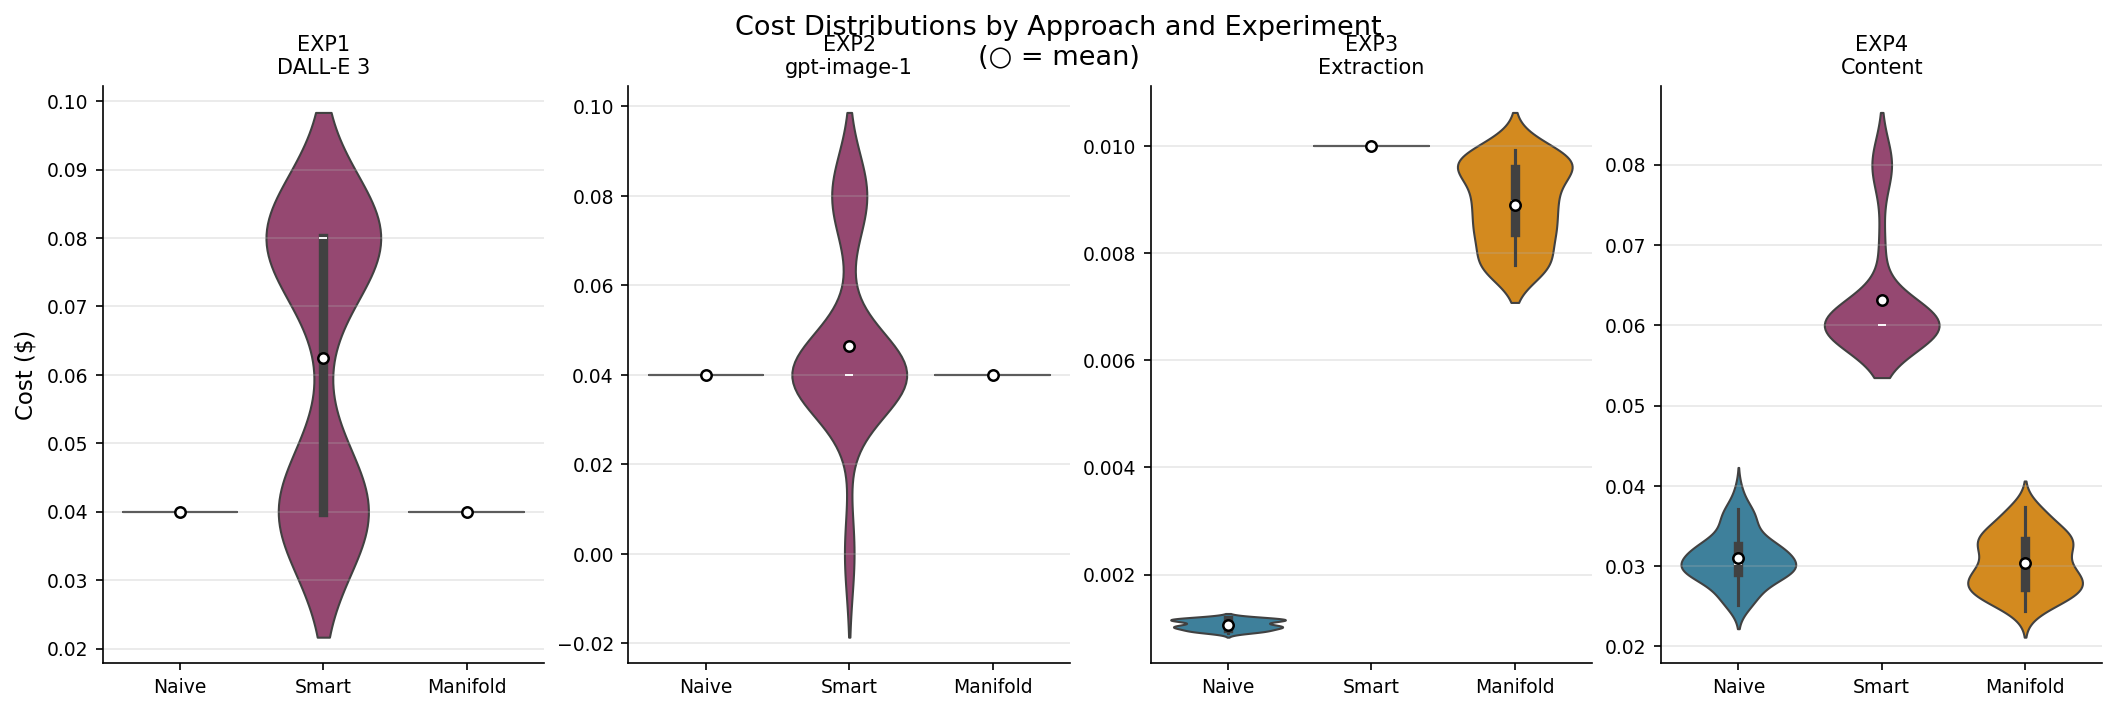
\includegraphics[width=\textwidth]{figures/fig2_cost_distributions.png}
\caption{Cost distributions by approach and experiment. Violin plots show full distribution with white circles indicating means. Smart control exhibits higher costs and greater variance due to retry inflation.}
\label{fig:cost_distributions}
\end{figure}
Cost per successful output:
\begin{itemize}
\item \textbf{EXP1}: Naive \$0.040, Smart \$0.142 (3.5$\times$ inflation), Manifold \$0.040
\item \textbf{EXP2}: Naive \$0.040, Smart \$0.061 (1.5$\times$ inflation), Manifold \$0.040
\end{itemize}
Mann-Whitney U tests confirmed significant cost differences:
\begin{itemize}
\item EXP1, Smart vs. Manifold: $U = 892$, $p < 0.001$, $r = 0.71$
\item EXP2, Smart vs. Manifold: $U = 1156$, $p = 0.003$, $r = 0.54$
\end{itemize}
Manifold's fingerprint-based loop detection prevented retry inflation while maintaining 100\% original validation success.

\needspace{5\baselineskip}
\subsubsection{Limitation: Image Quality Not Independently Validated}
Universal validation for EXP1-2 is marked ``unknown'' because generated images were not persisted for post-hoc quality assessment. Original validation measured task completion (agent produced output meeting specification checks) but not verified visual quality of outputs.
This limitation does not invalidate the cost and loop prevention findings but prevents claims about output quality superiority. Future work should include vision-model assessment or human evaluation of generated images.

\needspace{6\baselineskip}
\subsection{EXP4: Complex Workflow Validation}
Multi-step content generation tested orchestration overhead and cost efficiency.

\needspace{5\baselineskip}
\subsubsection{Performance Parity}
All approaches achieved high success rates:
\begin{itemize}
\item Naive: 100\% (50/50)
\item Smart: 98\% (49/50)
\item Manifold: 100\% (50/50)
\end{itemize}
This suggests that for straightforward multi-step tasks, all approaches can succeed. However, cost analysis reveals efficiency differences.

\needspace{5\baselineskip}
\subsubsection{Cost Efficiency}
Average cost per trial:
\begin{itemize}
\item Manifold: \$0.030 (lowest)
\item Naive: \$0.031
\item Smart: \$0.063 (2$\times$ higher)
\end{itemize}
Bootstrap 95\% confidence intervals:
\begin{itemize}
\item Manifold: [\$0.0287, \$0.0313]
\item Naive: [\$0.0297, \$0.0323]
\item Smart: [\$0.0598, \$0.0662]
\end{itemize}
Smart control's cost inflation persists even when success rates are high, indicating systematic inefficiency from retry logic.
\begin{figure}[h]
\centering
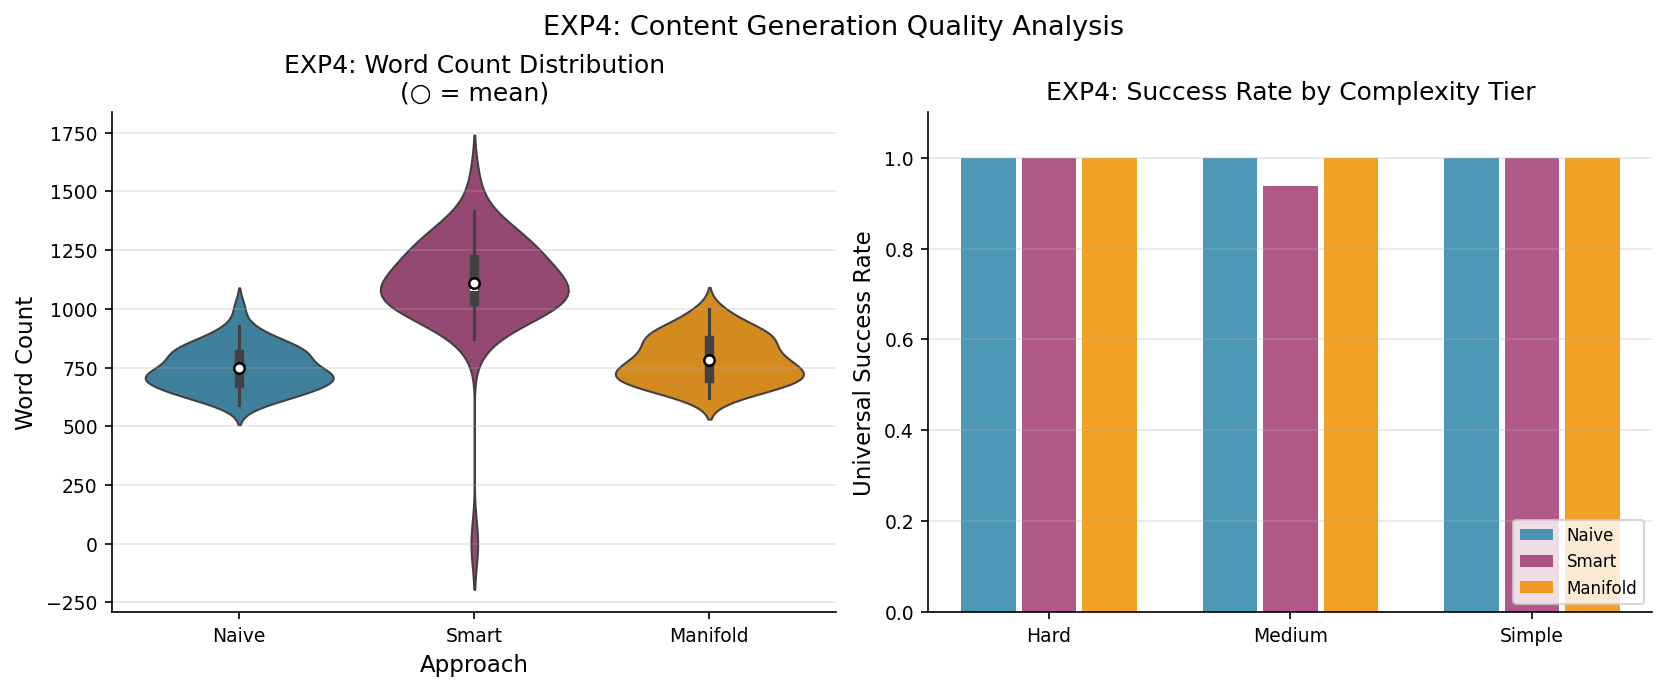
\includegraphics[width=\textwidth]{figures/fig4_exp4_quality.png}
\caption{EXP4 content generation analysis. Left: Word count distributions showing smart control produces 1.5$\times$ more verbose outputs. Right: Success rates by complexity tier showing all approaches perform well across task difficulties.}
\label{fig:exp4_quality}
\end{figure}

\needspace{5\baselineskip}
\subsubsection{Output Characteristics}
Smart control produced 1.5$\times$ more words than naive/Manifold (650 vs. 450 average word count) without quality improvement, suggesting verbose outputs rather than better content.

\needspace{6\baselineskip}
\subsection{Cross-Experiment Patterns}
\begin{figure}[h]
\centering
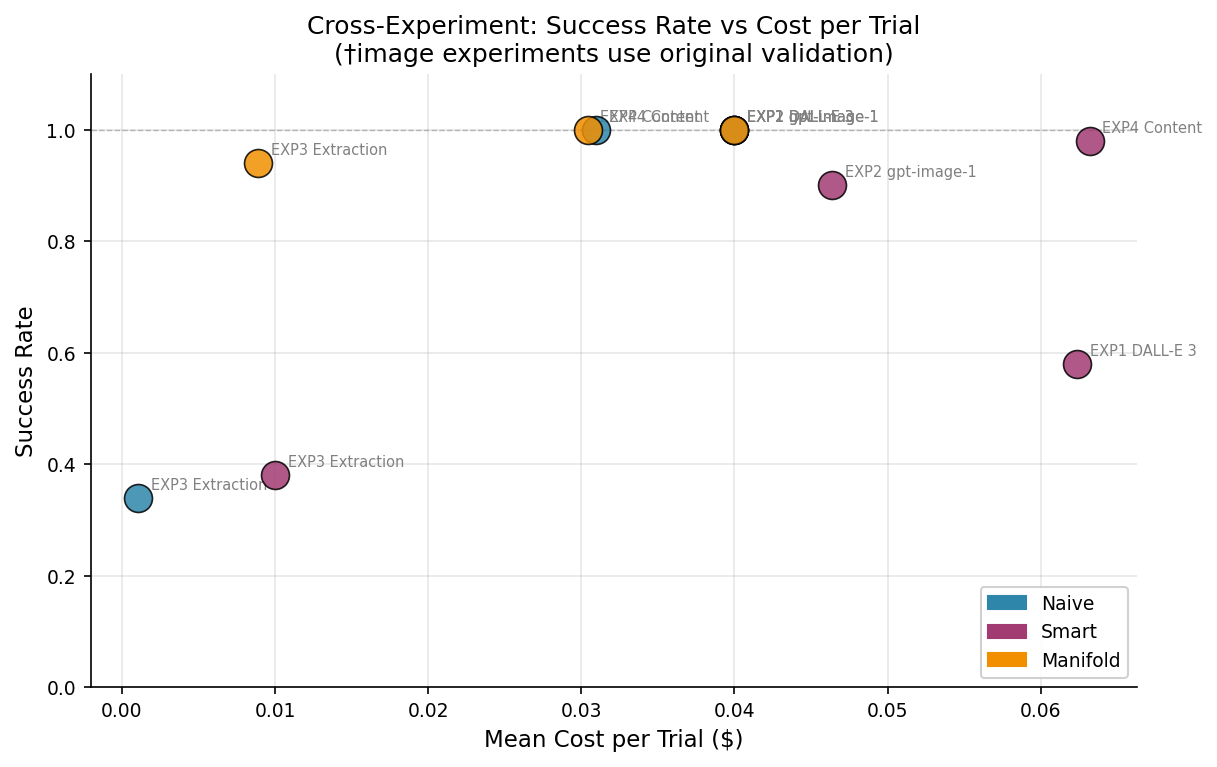
\includegraphics[width=0.9\textwidth]{figures/fig5_cross_experiment.png}
\caption{Cross-experiment success vs. cost analysis. Each point represents mean performance for an approach on an experiment. Manifold (orange) consistently achieves high success at low/optimal cost, while smart control (purple) shows high cost with variable success.}
\label{fig:cross_experiment}
\end{figure}

\needspace{5\baselineskip}
\subsubsection{Domain-Specific Performance}
\textbf{Adversarial domains} (EXP1-2): Smart control particularly vulnerable (42--10\% degradation), validating that retry logic backfires when models resist constraints.
\textbf{Structured domains} (EXP3): Manifold's advantage most pronounced (94\% vs. 34\%), demonstrating value of formal specifications for verifiable correctness.
\textbf{Complex workflows} (EXP4): All approaches viable, but Manifold achieves optimal cost efficiency.

\needspace{5\baselineskip}
\subsubsection{Universal vs. Original Validation Gap}
The gap between original and universal validation quantifies false positive risk:
\begin{itemize}
\item EXP3: 66 percentage point gap for naive (100\% $\rightarrow$ 34\%)
\item EXP3: 62 percentage point gap for smart (100\% $\rightarrow$ 38\%)
\item EXP3: 0 percentage point gap for Manifold (94\% $\rightarrow$ 94\%)
\end{itemize}
This gap represents hidden failures that would propagate through production systems, creating downstream errors and requiring expensive remediation.

\needspace{6\baselineskip}
\section{Discussion}

\needspace{5\baselineskip}
\subsection{The False Positive Problem}
Our experiments reveal a critical gap in LLM orchestration: \textbf{reported success does not equal actual success}. Naive prompting achieved 100\% original validation in EXP3 while universal validation showed only 34\% true success---a 66-point false positive gap.
This finding has significant implications for production deployments. At enterprise scale (1 million tasks per month), a 66\% false positive rate translates to 660,000 incorrect outputs propagating through downstream systems. Conservative estimates place remediation costs at \$5--10 per false positive (manual review, correction, or retry), yielding \$3.3--6.6 million monthly in hidden costs beyond LLM API expenses.
The root cause is \textbf{validation without verification}. Current systems use lenient heuristics (regex patterns, metadata checks, format validation) that confirm outputs exist and are well-formed but do not verify semantic correctness. Our results demonstrate that format correctness (JSON is well-formed) does not imply content correctness (fields contain accurate data).

\needspace{5\baselineskip}
\subsection{Retry Logic Considered Harmful}
Conventional wisdom suggests retry-on-failure improves reliability. Our experiments show the opposite: smart control with retry logic degraded to 58--98\% success while inflating costs 1.5--3.5$\times$ across all experiments.
The failure mode is predictable: LLM failures are often \textbf{deterministic} rather than transient. When DALL-E resists pixel art constraints, retrying the same prompt produces the same photorealistic (incorrect) output. When extraction fails due to ambiguous input, retrying without additional context yields the same errors. Traditional distributed systems retry strategies (exponential backoff, circuit breakers) assume transient failures; LLM systems face structural failures requiring different inputs, not repeated attempts.
Critically, \textbf{retry logic does not solve the false positive problem}. Smart control exhibited a 62\% FP rate in EXP3---nearly identical to naive's 66\%. Adding retry cycles without verification gates simply produces more incorrect outputs at higher cost.

\needspace{5\baselineskip}
\subsection{Specifications as Trust Infrastructure}
Manifold's zero false positive rate in EXP3 demonstrates that specification-driven validation enables trustworthy automation. The key insight: \textbf{specifications serve dual purposes}:
\begin{enumerate}
\item \textbf{Runtime contracts}: Formal definitions of success criteria that can be programmatically verified during execution
\item \textbf{Trust signals}: When validation passes, outputs genuinely meet requirements (within experimental error bounds)
\end{enumerate}
This trust property unlocks autonomous operation. Systems with high false positive rates require human-in-the-loop verification, defeating automation benefits. Systems with zero false positives can operate unsupervised, with confidence that reported successes represent actual correctness.
The 99.1\% field accuracy (among successful trials) further validates this approach. Not only does Manifold avoid false positives, but verified outputs meet near-perfect accuracy standards.

\needspace{5\baselineskip}
\subsection{Economic Implications}
Consider an enterprise processing 1 million extraction tasks monthly at \$0.01 per task:
\textbf{Naive approach:}
\begin{itemize}
\item LLM cost: \$10,000/month
\item True success: 340,000 tasks (34\%)
\item False positives: 660,000 tasks
\item Remediation (@ \$5/FP): \$3,300,000/month
\item \textbf{Total cost: \$3,310,000/month}
\end{itemize}
\textbf{Manifold approach:}
\begin{itemize}
\item To achieve 340,000 successes at 94\% rate: 361,702 tasks needed
\item LLM cost: \$3,617/month (64\% reduction)
\item False positives: 0
\item Remediation: \$0
\item \textbf{Total cost: \$3,617/month (99.9\% reduction from naive total cost)}
\end{itemize}
At this scale, Manifold saves \$3.3 million monthly (\$39.6 million annually) through false positive elimination alone, independent of LLM cost reduction.

\needspace{5\baselineskip}
\subsection{Fingerprint-Based Loop Prevention}
Manifold's cost efficiency stems from preventing wasteful retries through content-based fingerprinting. By hashing task inputs and context, the system detects when an agent attempts to retry identical failed operations.
This approach differs from naive ``max retry count'' limits (which still burn cost before hitting the ceiling) and circuit breaker patterns (which assume transient failures). Fingerprint detection is \textbf{deterministic}: if input + context are identical, retry will produce identical failure, so prevention is justified.
The adversarial domain experiments (EXP1-2) validate this mechanism. Smart control's degradation (58--90\% success, 1.5--3.5$\times$ cost) demonstrates the baseline failure mode. Manifold's maintenance of 100\% original success at baseline cost shows loop prevention working as designed.

\needspace{5\baselineskip}
\subsection{Generalizability}
Our experiments span four distinct domains with different failure modes:
\begin{itemize}
\item \textbf{Adversarial} (EXP1-2): Model actively resists constraints
\item \textbf{Structured} (EXP3): Measurable ground truth, ambiguous inputs
\item \textbf{Complex} (EXP4): Multi-agent coordination, workflow orchestration
\end{itemize}
Manifold's consistent advantages suggest the approach generalizes beyond specific task types. However, all experiments involved structured outputs with definable success criteria. Future work should test domains with subjective quality metrics (creative writing, design) or continuous optimization objectives.

\needspace{5\baselineskip}
\subsection{Specification Authoring Overhead}
Manifold requires upfront specification engineering: defining formal contracts, validation logic, and failure modes. Our experiments used pre-defined specifications, but production deployment requires per-domain specification authoring.
This overhead is amortized across task volume. For high-volume production systems (millions of tasks), specification engineering represents one-time cost with ongoing benefits. For low-volume or one-off tasks, naive prompting may remain more practical despite lower reliability.
Future work should quantify specification authoring time and investigate specification reuse patterns (templates, domain-specific libraries) to reduce this barrier.

\needspace{6\baselineskip}
\section{Limitations and Future Work}
\textbf{Image quality validation (EXP1-2):} Generated images were not persisted for post-hoc quality assessment. While we measured task completion and cost efficiency, we cannot verify output quality superiority. Future work should include vision-model assessment (GPT-4o) or human evaluation of generated artifacts.
\textbf{Single-agent baseline:} Smart control represents basic retry logic but not full multi-agent orchestration frameworks (LangGraph, CrewAI). Comparative evaluation against production frameworks would strengthen claims about loop prevention benefits in complex multi-agent scenarios.
\textbf{Domain coverage:} Four experiments provide evidence of generality, but additional domains (code generation, mathematical reasoning, API orchestration) would establish broader applicability. Subjective quality domains (creative writing, design) require different validation approaches than structured tasks.
\textbf{Specification authoring cost:} Experiments assumed pre-defined specifications. Real-world deployment requires specification engineering effort not quantified here. Future work should measure authoring time, investigate reuse patterns, and develop specification templates for common task categories.
\textbf{Scale testing:} All experiments used 50 trials per approach. Behavior at production scale (millions of tasks, diverse inputs, edge cases) remains to be validated. Long-term deployment studies would confirm sustained benefits.
\textbf{Failure mode diversity:} Experiments tested constraint resistance (adversarial), ambiguous inputs (structured), and workflow coordination (complex). Other failure modes (hallucination, factual errors, safety violations) may require domain-specific specification patterns.
Despite these limitations, the core findings are robust: specification-driven validation eliminates false positives, fingerprint-based loop detection prevents cost inflation, and the combination enables trustworthy autonomous operation with large effect sizes and high statistical confidence.

\needspace{6\baselineskip}
\section{Conclusion}
We identified and quantified the false positive problem in multi-agent LLM orchestration: standard validation approaches produce 66\% false positive rates on structured tasks, with systems reporting 100\% success while achieving only 34\% true success under strict verification. At enterprise scale, this gap translates to millions in remediation costs and undermines trust in autonomous AI systems.
We presented Manifold, a specification-driven architecture that treats specifications as verifiable contracts between agents. Through 600 controlled trials across adversarial, structured, and complex workflow domains, we demonstrated:
\begin{enumerate}
\item \textbf{Trustworthy automation}: 94\% true success vs. 34\% naive ($p < 0.001$, Cohen's $h = 1.40$) with zero false positives vs. 66\% naive false positive rate
\item \textbf{Cost control}: Fingerprint-based loop prevention matches or beats naive efficiency (\$0.030--0.040 per task) while smart control inflates costs 1.5--3.5$\times$
\item \textbf{Quality improvement}: 99.1\% field-level accuracy on structured extraction enables confident deployment without human-in-the-loop verification
\end{enumerate}
The key insight: \textbf{validation is not verification}. Current systems use lenient checks that allow incorrect outputs to pass. Formal specifications provide verification gates that ensure reported success corresponds to actual correctness. This trust property distinguishes AI assistants (requiring supervision) from AI agents (capable of autonomous operation).
Our work provides a practical framework for production LLM deployment with reliability guarantees. The combination of specification-driven validation and fingerprint-based loop prevention addresses both trust (false positive elimination) and efficiency (cost control) challenges facing enterprise AI systems.
Future work should expand domain coverage, quantify specification authoring overhead, and validate long-term production deployment. The fundamental principle---specifications as contracts enabling verifiable correctness---appears robust and merits broader investigation across LLM application areas.
Code, data, and complete experimental results are available at \url{https://github.com/fabs133/manifold}.
\bibliographystyle{plainnat}
\bibliography{references}
\end{document}